\documentclass{article}
\usepackage{graphicx} % Required for inserting images

\title{The CLASS-ification of Raisins: Capitalism Reaches Our Farms}
\author{Jonathan Ferdinand, Devina Gera, Archimedes Li, Henry Liu, \\Katherine Shi, Sam Stevens}
\date{\today}

\begin{document}

\maketitle

\section{Introduction}

We use and compare two different classification models, k-nearest neighbors and decision trees.  Each model is tasked with classifying raisins into the Kecimen or Besni class based on a set of 7 independent variables (see Data Description).

The k-nearest neighbors (kNN) model works by finding the k closest data points using Euclidean distance, and selects the most common class among those neighbors.  Some assumptions for the kNN to work well is that all features are normalized, and that there are no unnecessary features.  Some benefits to the kNN model is that it is non-parametric, which makes it flexible to different data distributions.  However, it has a major drawback with computational cost, since it needs to calculate the distance with every single point for each prediction.

The decision tree model recursively splits the data according to a threshold of a variable.  Because every decision is explicitly listed and the decision tree can be clearly graphically visualized, the decision tree has a high interpretability.  They are also robust to extraneous features and outliers, thus no data assumptions are necessary.  However, decision trees are prone to overfitting, so it is important to limit the number of branches through methods like pruning.


\section{Data Description}
Our dataset consisted of 900 instances, each pertaining to an image of a raisin. The dataset extracted 7 features (listed below) from each of the images, along with a label of either Kecimen or Besni, which are the raisin types (and the label that we classified between). There were 450 instances for each label.

\begin{enumerate}
    \item Area - Gives the number of pixels within the boundaries of the raisin.
\item Major axis length - Gives the pixel length of the main axis, which is the longest line that can be drawn on the raisin.

\item Minor axis length - Gives the pixel length of the small axis, which is the shortest line that can be drawn on the raisin.

\item Eccentricity - It gives a measure of the eccentricity of the ellipse, which has the same moments as raisins.  Values closer to 0 indicate the raisin is more circular, and values closer to 1 indicate that the raisin is more elongated.

\item Convex area - Gives the number of pixels of the smallest convex shell of the region formed by the raisin.

\item Extent - Gives the ratio of the region formed by the raisin to the total pixels in the bounding box.  Ranges from 0 to 1.

\item Perimeter - It measures the environment by calculating the distance between the boundaries of the raisin and the pixels around it.

While looking through the data, we saw no obvious outliers, so we did not need to perform any form of data cleaning. 

Our data was found from Kaggle \cite{Raisin}. 

\end{enumerate}

\section{Analysis}

We first shuffled the data to ensure raisin classes were well mixed rather than separated. We then split our data, using 70\% of the data for training and the remaining 30\% for testing. We also normalized the data between the ranges of 0 and 1 for the kNN model. 

We can see the diagonal plots for the model in figure 1. There is a strong correlation between the AxisLengths, perimeter, and  Area, which makes sense. There is weak correlation between Extent and Area, Eccentricity and MinorAxisLength, (which is surprising considering that there is statistically significant correlation between eccentricity and MajorAxisLength), Extent and ConvexArea, Extent and MinorAxisLength. The remaining variables have some level of statistically significant correlation( refer to Fig \ref{fig:enter-label} for more details)

\begin{figure}[h]
    \centering
    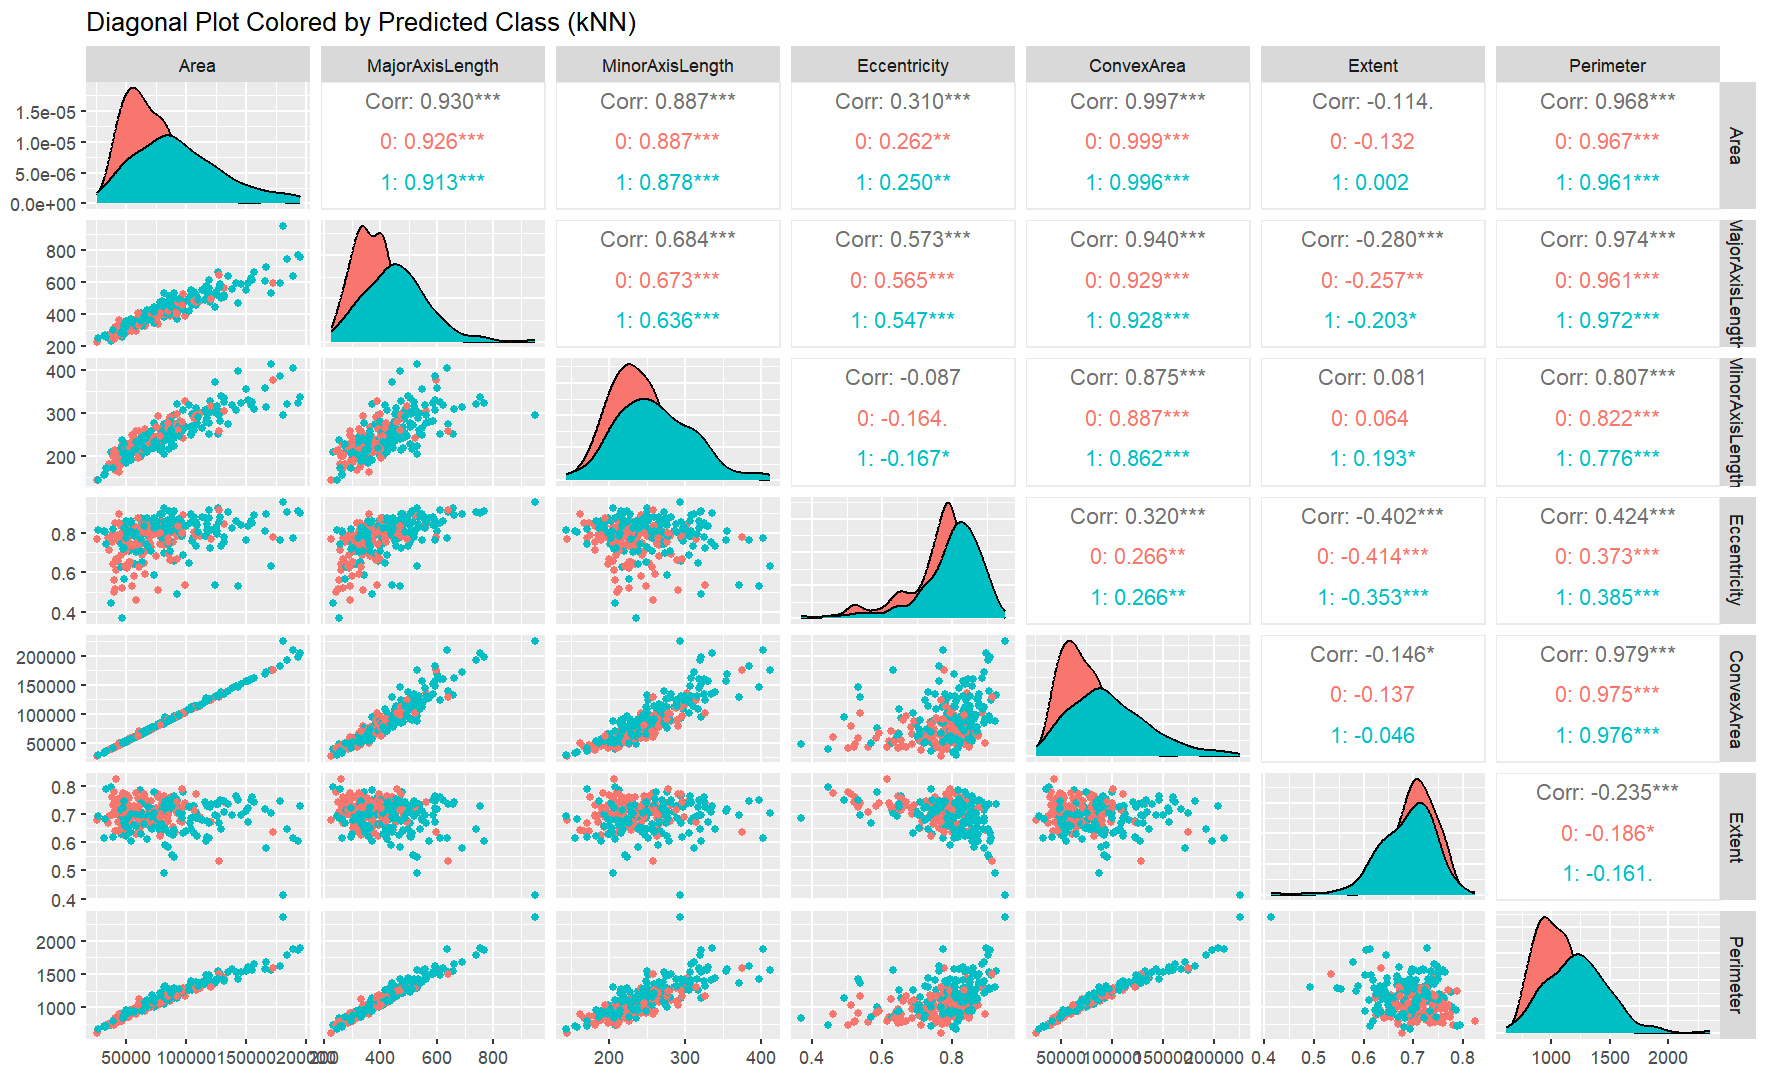
\includegraphics[width=1\linewidth]{diagonal.png}
    \caption{Diagonal plots showing the correlation between all the combinations of predicting variables for the decision tree.}
    \label{fig:enter-label}
\end{figure}

We used trial and error to find that $k = 5$ worked the best for our model with an accuracy of $85.9\%$. Figure \ref{fig:enter-label} also supports our assumption that certain features are grouped for different types of Raisin. The histograms along the diagonal show differing mean and standard deviation between the class of raisin and feature for all features other than extent and eccentricity. 


\newpage
\section{Model Evaluation}

\subsection{Decision Tree Model}
We trained our decision tree to find the split points shown in figure 2.

\begin{figure}[h]
    \centering
    \includegraphics[width=0.7\linewidth]{twee.png}
    \caption{Diagram of decision choices at each level of trained decision tree}
    \label{fig:enter-label}
\end{figure}

Since decision trees are able to run on all features, we did not need to perform any subset selection.

We found the following confusion matrix on the test data.

\begin{verbatim}
              Reference
Prediction   0   1
         0 113  20
         1  15 123
\end{verbatim}

From the confusion matrix, we determined the accuracy to be 0.87.

Furthermore, we found the following metrics for precision, recall, and F1-score.

For the Kecimen class, we found

\begin{enumerate}
    \item Precision: 0.849

    \item Recall: 0.882

    \item F1-score: 0.865
\end{enumerate}

For the Besni class, we found

\begin{enumerate}
    \item Precision: 0.891

    \item Recall: 0.860

    \item F1-Score: 0.875
\end{enumerate}

\newpage 

\subsection{kNN Model}
We first ran our kNN without doing subset selection and found an accuracy of 85\% on the testing data. We then wanted to refine our model using subset selection.

To ensure optimality of features for using a kNN algorithm, we ran subset selection with 10-fold cross validation to determine the most impactful features.

We can see the output below.

\begin{verbatim}
    Variables   RMSE Rsquared    MAE  RMSESD RsquaredSD   MAESD Selected
         1 0.3441   0.5297 0.2116 0.04560    0.11039 0.03404         
         2 0.3234   0.5815 0.1957 0.04344    0.10753 0.03299        *
         3 0.3269   0.5735 0.1970 0.03932    0.09452 0.02596         
         4 0.3324   0.5603 0.2000 0.04148    0.09800 0.02525         
         5 0.3416   0.5366 0.2129 0.04203    0.10279 0.02956         
         6 0.3427   0.5334 0.2131 0.03537    0.08722 0.02469         
         7 0.3298   0.5652 0.2041 0.04100    0.10170 0.03158 
\end{verbatim}

From the output, we saw that all predictor variables had similar impact on the final prediction, and after tests with various subsets, we determined that using all features for the kNN model was optimal.

Our kNN found an accuracy of 0.8593 on the testing data, with the confusion matrix shown below.

\begin{verbatim}
              Reference
Prediction   0   1
         0 110  20
         1  18 122
\end{verbatim}

where $0$ pertains to Kecimen and $1$ is Besni. We can use these metrics to calculate the precision, recall, and F1-score of our model as well.

For the Kecimen class, we found

\begin{enumerate}
    \item Precision: 0.846

    \item Recall: 0.859

    \item F1-score: 0.853
\end{enumerate}

For the Besni class, we found

\begin{enumerate}
    \item Precision: 0.871

    \item Recall: 0.859

    \item F1-Score 0.868
\end{enumerate}

Overall, we see good performance from our kNN Model, with high precision, recall, F1-score, and accuracy.

The entire output can be found in Appendix B, along with our code in Appendix A.

\subsection{Comparison}

Overall, we found better accuracy using the decision tree, as well as better precision, recall, and F1-score on average. This indicates that the decision tree model is more optimal for this dataset compared to the kNN model.



\section{Conclusion}

Overall, we found good results with both the kNN model and the decision tree model. We saw slightly higher accuracy using the decision tree, with 87\%, compared to 86\% using the kNN. The robustness of both models and being able to take into account all features of the dataset likely led to good performance. In addition, we saw higher precision and recall metrics with the decision tree as well, which may indicate that the data is not necessarily partitioned in space as well as we first thought.

Finally, we are able to interpret the decisions of the tree model much better than of the kNN. Future steps may include testing with more robust models such as neural networks, or implementing ensemble methods such as random forests.

\begin{thebibliography}{9}

\bibitem{STHDA}
Lateef, Z. (2022, March 29). \emph{KNN Algorithm: A practical implementation of KNN algorithm in R.} Edureka. https://www.edureka.co/blog/knn-algorithm-in-r/

\bibitem{Raisin}
\emph{Raisin binary classification}. (2024, February 11). Kaggle. https://www.kaggle.com/datasets/nimapourmoradi/raisin-binary-classification/data


\bibitem{advert}
Blog, G. (2020, June 26). \emph{Best way to learn kNN Algorithm using R Programming}. Analytics Vidhya. https://www.analyticsvidhya.com/blog/2015/08/learning-concept-knn-algorithms-programming/

\newpage

\section{Appendix A: Code}

\begin{verbatim}
    library("class")
library("caret")
library("rpart")
library("rpart.plot")
library("class")
library("ggplot2")
library("tree")
library("randomForest")
library(GGally

# Load data set
raisins <- read.csv("data/Raisin_Dataset.csv")
raisins <- na.omit(raisins) # Remove missing values

# Convert Class to binary (Besni = 1, Kecimen = 0)
raisins$Class <- ifelse(raisins$Class == "Besni", 1, 0)

# Shuffle data
set.seed(456)
train_idx  <- sample(1:nrow(raisins),size = 0.7 * nrow(raisins))
train_data  <- raisins[train_idx,]
test_data  <-  raisins[-train_idx,]

tree_model  <-  rpart(Class ~ .,data=train_data)

#tree_pred  <- predict(tree_model, data, type = "class")

summary(tree_model)
rpart.plot(tree_model)

# Normalize the features (KNN performs better with scaled data)
normalize <- function(x) {
  return ((x - min(x)) / (max(x) - min(x)))
}

raisins_norm <- as.data.frame(lapply(raisins[1:7], normalize))
raisins_labels <- raisins$Class

train_data <- raisins_norm[train_idx, ]
test_data <- raisins_norm[-train_idx, ]
train_labels <- raisins_labels[train_idx]
test_labels <- raisins_labels[-train_idx]

# Print the results
print(rfe_result)
plot(rfe_result)

train_subset <- train_data[, c("MajorAxisLength", "Extent", "Eccentricity", "Area", "ConvexArea")]
test_subset <- test_data[, c("MajorAxisLength", "Extent", "Eccentricity", "Area", "ConvexArea")]
knn_pred  <- knn(train = train_data, test = test_data, cl = train_labels)

summary(knn_pred)

confusionMatrix(knn_pred, as.factor(test_labels))

train_idx  <- sample(1:nrow(raisins),size = 0.7 * nrow(raisins))
train_data  <- raisins[train_idx,]
test_data  <-  raisins[-train_idx,]

tree_model  <-  rpart(Class ~ .,data=train_data)

tree_pred  <- predict(tree_model, test_data, type = "vector")

confusion_matrix <- table(Predicted = tree_pred, Actual = as.factor(test_labels))
print(confusion_matrix)

## --- Create DataFrames for Plotting ---
#knn_df <- data.frame(train_data, Predicted = knn_pred)
#tree_df <- data.frame(features, Predicted = tree_pred)  # unscaled for readability
#
## --- Pair Plot for k-NN Output ---
#ggpairs(knn_df, mapping = aes(color = Predicted), 
#        columns = 1:4, title = "k-NN Classification (Pair Plot)")
#
## --- Pair Plot for Decision Tree Output ---
#ggpairs(tree_df, mapping = aes(color = Predicted), 
#        columns = 1:4, title = "Decision Tree Classification (Pair Plot)")
#
#

plot_data <- test_data[, 1:7]
plot_data$Predicted <- knn_pred
ggpairs(plot_data, mapping = aes(color = Predicted),
        columns = 1:4,   # only the features in the plot
        title = "Diagonal Plot Colored by Predicted Class (kNN)")


\end{verbatim}
\newpage
\section{Appendix B: Code output}
\begin{verbatim}
    Call:
rpart(formula = Class ~ ., data = train_data)
  n= 630 

          CP nsplit rel error    xerror        xstd
1 0.54610840      0 1.0000000 1.0033964 0.002067902
2 0.02777736      1 0.4538916 0.4747240 0.040191848
3 0.02592519      2 0.4261142 0.4841338 0.039782251
4 0.01189352      3 0.4001890 0.4482840 0.036409638
5 0.01171031      6 0.3645085 0.4586555 0.038476170
6 0.01066365      7 0.3527982 0.4656669 0.039548677
7 0.01000000      8 0.3421345 0.4704892 0.040023798

Variable importance
MajorAxisLength       Perimeter      ConvexArea            Area    Eccentricity MinorAxisLength 
             22              21              18              17              11              11 

Node number 1: 630 observations,    complexity param=0.5461084
  mean=0.4888889, MSE=0.2498765 
  left son=2 (351 obs) right son=3 (279 obs)
  Primary splits:
      MajorAxisLength < 424.3492  to the left,  improve=0.5461084, (0 missing)
      Perimeter       < 1122.496  to the left,  improve=0.5282751, (0 missing)
      ConvexArea      < 88202.5   to the left,  improve=0.4382655, (0 missing)
      Area            < 90276.5   to the left,  improve=0.4107736, (0 missing)
      Eccentricity    < 0.8010812 to the left,  improve=0.2234476, (0 missing)
  Surrogate splits:
      Perimeter       < 1157.055  to the left,  agree=0.959, adj=0.907, (0 split)
      ConvexArea      < 84535.5   to the left,  agree=0.910, adj=0.796, (0 split)
      Area            < 79741.5   to the left,  agree=0.902, adj=0.778, (0 split)
      Eccentricity    < 0.8061662 to the left,  agree=0.771, adj=0.484, (0 split)
      MinorAxisLength < 258.6526  to the left,  agree=0.765, adj=0.470, (0 split)

Node number 2: 351 observations,    complexity param=0.02592519
  mean=0.1595442, MSE=0.1340898 
  left son=4 (319 obs) right son=5 (32 obs)
  Primary splits:
      Perimeter       < 1122.496  to the left,  improve=0.08671317, (0 missing)
      MajorAxisLength < 355.0498  to the left,  improve=0.07616695, (0 missing)
      ConvexArea      < 88202.5   to the left,  improve=0.04672551, (0 missing)
      Area            < 47107     to the left,  improve=0.03522397, (0 missing)
      Eccentricity    < 0.802124  to the left,  improve=0.03064046, (0 missing)
  Surrogate splits:
      ConvexArea      < 82196.5   to the left,  agree=0.954, adj=0.500, (0 split)
      Area            < 83150     to the left,  agree=0.952, adj=0.469, (0 split)
      MinorAxisLength < 292.1377  to the left,  agree=0.932, adj=0.250, (0 split)
      MajorAxisLength < 409.2138  to the left,  agree=0.920, adj=0.125, (0 split)

Node number 3: 279 observations,    complexity param=0.02777736
  mean=0.9032258, MSE=0.08740895 
  left son=6 (83 obs) right son=7 (196 obs)
  Primary splits:
      MajorAxisLength < 466.3234  to the left,  improve=0.17930690, (0 missing)
      Perimeter       < 1259.692  to the left,  improve=0.16638530, (0 missing)
      ConvexArea      < 99619.5   to the left,  improve=0.11406260, (0 missing)
      Area            < 97201.5   to the left,  improve=0.09902263, (0 missing)
      Eccentricity    < 0.8526956 to the left,  improve=0.04961900, (0 missing)
  Surrogate splits:
      Perimeter       < 1255.784  to the left,  agree=0.907, adj=0.687, (0 split)
      Area            < 94246.5   to the left,  agree=0.849, adj=0.494, (0 split)
      ConvexArea      < 95650.5   to the left,  agree=0.846, adj=0.482, (0 split)
      MinorAxisLength < 237.3404  to the left,  agree=0.728, adj=0.084, (0 split)

Node number 4: 319 observations,    complexity param=0.01171031
  mean=0.1253918, MSE=0.1096687 
  left son=8 (259 obs) right son=9 (60 obs)
  Primary splits:
      Eccentricity    < 0.8156898 to the left,  improve=0.05269399, (0 missing)
      MajorAxisLength < 355.0498  to the left,  improve=0.05195481, (0 missing)
      Perimeter       < 919.2315  to the left,  improve=0.04569989, (0 missing)
      ConvexArea      < 49543.5   to the left,  improve=0.03026478, (0 missing)
      Area            < 47107     to the left,  improve=0.02823835, (0 missing)
  Surrogate splits:
      Extent          < 0.6449237 to the right, agree=0.843, adj=0.167, (0 split)
      MajorAxisLength < 408.9334  to the left,  agree=0.837, adj=0.133, (0 split)
      MinorAxisLength < 198.4415  to the right, agree=0.821, adj=0.050, (0 split)

Node number 5: 32 observations
  mean=0.5, MSE=0.25 

Node number 6: 83 observations,    complexity param=0.01189352
  mean=0.7108434, MSE=0.2055451 
  left son=12 (66 obs) right son=13 (17 obs)
  Primary splits:
      Eccentricity    < 0.852826  to the left,  improve=0.10477660, (0 missing)
      Area            < 82689     to the right, improve=0.07435852, (0 missing)
      MinorAxisLength < 227.4308  to the right, improve=0.06214689, (0 missing)
      ConvexArea      < 79155.5   to the right, improve=0.05572324, (0 missing)
      Perimeter       < 1262.853  to the left,  improve=0.04338983, (0 missing)
  Surrogate splits:
      MinorAxisLength < 237.0866  to the right, agree=0.928, adj=0.647, (0 split)
      Area            < 79403     to the right, agree=0.880, adj=0.412, (0 split)
      ConvexArea      < 78854     to the right, agree=0.880, adj=0.412, (0 split)
      Perimeter       < 1109.018  to the right, agree=0.831, adj=0.176, (0 split)

Node number 7: 196 observations
  mean=0.9846939, MSE=0.01507185 

Node number 8: 259 observations
  mean=0.08880309, MSE=0.0809171 

Node number 9: 60 observations,    complexity param=0.01066365
  mean=0.2833333, MSE=0.2030556 
  left son=18 (49 obs) right son=19 (11 obs)
  Primary splits:
      Perimeter       < 1071.628  to the left,  improve=0.13778620, (0 missing)
      ConvexArea      < 69528     to the left,  improve=0.08866405, (0 missing)
      Area            < 44995     to the left,  improve=0.07906977, (0 missing)
      MinorAxisLength < 219.037   to the left,  improve=0.07596019, (0 missing)
      MajorAxisLength < 359.6973  to the left,  improve=0.07363650, (0 missing)
  Surrogate splits:
      Area            < 65188     to the left,  agree=0.950, adj=0.727, (0 split)
      ConvexArea      < 68090.5   to the left,  agree=0.950, adj=0.727, (0 split)
      MinorAxisLength < 219.037   to the left,  agree=0.933, adj=0.636, (0 split)
      MajorAxisLength < 408.0757  to the left,  agree=0.900, adj=0.455, (0 split)
      Eccentricity    < 0.8162848 to the right, agree=0.850, adj=0.182, (0 split)

Node number 12: 66 observations,    complexity param=0.01189352
  mean=0.6363636, MSE=0.231405 
  left son=24 (25 obs) right son=25 (41 obs)
  Primary splits:
      Perimeter       < 1182.066  to the left,  improve=0.10160280, (0 missing)
      Eccentricity    < 0.8404073 to the right, improve=0.08897783, (0 missing)
      MajorAxisLength < 440.9799  to the right, improve=0.05982906, (0 missing)
      ConvexArea      < 99837     to the left,  improve=0.05252101, (0 missing)
      MinorAxisLength < 267.4984  to the left,  improve=0.04111842, (0 missing)
  Surrogate splits:
      ConvexArea      < 87756.5   to the left,  agree=0.848, adj=0.60, (0 split)
      Area            < 85015.5   to the left,  agree=0.818, adj=0.52, (0 split)
      MinorAxisLength < 253.2314  to the left,  agree=0.803, adj=0.48, (0 split)
      MajorAxisLength < 435.8667  to the left,  agree=0.758, adj=0.36, (0 split)
      Eccentricity    < 0.8089715 to the right, agree=0.727, adj=0.28, (0 split)

Node number 13: 17 observations
  mean=1, MSE=0 

Node number 18: 49 observations
  mean=0.2040816, MSE=0.1624323 

Node number 19: 11 observations
  mean=0.6363636, MSE=0.231405 

Node number 24: 25 observations,    complexity param=0.01189352
  mean=0.44, MSE=0.2464 
  left son=48 (8 obs) right son=49 (17 obs)
  Primary splits:
      MajorAxisLength < 440.2683  to the right, improve=0.3697479, (0 missing)
      Area            < 83993     to the right, improve=0.1558442, (0 missing)
      ConvexArea      < 90437.5   to the right, improve=0.1393527, (0 missing)
      Perimeter       < 1176.257  to the right, improve=0.1393527, (0 missing)
      Eccentricity    < 0.8395464 to the right, improve=0.1393527, (0 missing)
  Surrogate splits:
      Perimeter    < 1178.441  to the right, agree=0.84, adj=0.500, (0 split)
      Area         < 83993     to the right, agree=0.76, adj=0.250, (0 split)
      ConvexArea   < 90810     to the right, agree=0.76, adj=0.250, (0 split)
      Eccentricity < 0.8395464 to the right, agree=0.72, adj=0.125, (0 split)

Node number 25: 41 observations
  mean=0.7560976, MSE=0.184414 

Node number 48: 8 observations
  mean=0, MSE=0 

Node number 49: 17 observations
  mean=0.6470588, MSE=0.2283737 

  0   1 
130 140 
Confusion Matrix and Statistics

          Reference
Prediction   0   1
         0 110  20
         1  18 122
                                         
               Accuracy : 0.8593         
                 95% CI : (0.812, 0.8984)
    No Information Rate : 0.5259         
    P-Value [Acc > NIR] : <2e-16         
                                         
                  Kappa : 0.718          
                                         
 Mcnemar's Test P-Value : 0.8711         
                                         
            Sensitivity : 0.8594         
            Specificity : 0.8592         
         Pos Pred Value : 0.8462         
         Neg Pred Value : 0.8714         
             Prevalence : 0.4741         
         Detection Rate : 0.4074         
   Detection Prevalence : 0.4815         
      Balanced Accuracy : 0.8593         
                                         
       'Positive' Class : 0              

\end{verbatim}

\end{thebibliography}

\end{document}
